\chapter{Pruebas Locales}

\section{Ejecutar el sistema de manera local (Spring)}

\subsection{Spring tools suite}
Para ejecutar el proyecto de manera local se tienen que seguir los siguientes pasos:
\begin{enumerate}
    \item Se tiene que ejecutar el siguiente comando: git clone https://github.com/SoftwareEngineerESCOM/APMS-Server.git este comando hará una copia del proyecto del sistema.
    \item Después se tiene que ejecutar en la carpeta el ejecutable ./STS que está en la caperta springTools como lo muestra la figura 6.1.
    \item Se abrirá una pantalla como la de la figura 6.2.
    \item Se tiene que importar el proyecto a spring tools suite que descargamos desde github como lo muestra la figura 6.3
    \item Una vez importado se tiene que oprimir el botón de la figura 6.4 y seleccionamos la opción de Spring boot App.
    \item Se abrirá la terminal de spring boot suite y esperaremos hasta que apareza el mensaje de la figura 6.5.
    \item Una vez hecho esto tendremos nuestro servicio de Api Rest de manera local.
\end{enumerate}


\begin{figure}[H]
	\centering
	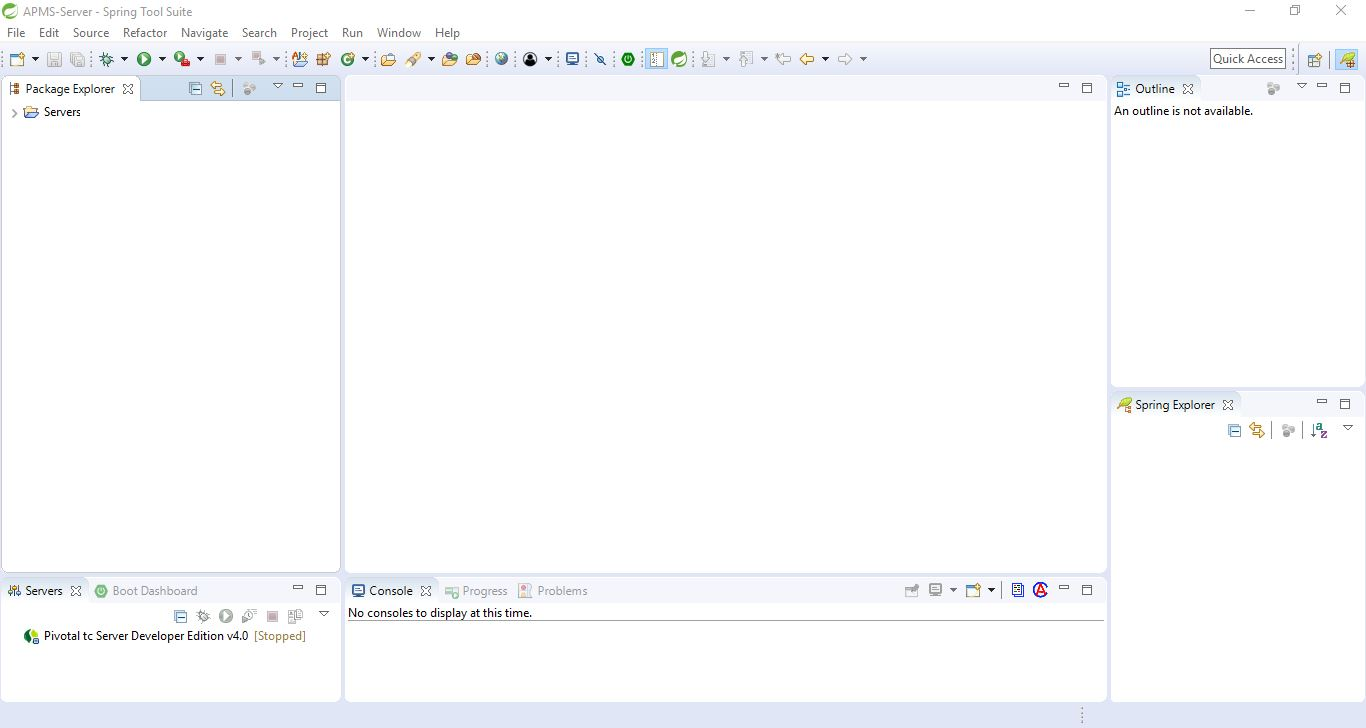
\includegraphics[width=0.7\linewidth]{images/tecnologias/spring.JPG}
	\caption{Entorno de desarrollo spring boot suite.}
\end{figure}


\begin{figure}[H]
	\centering
	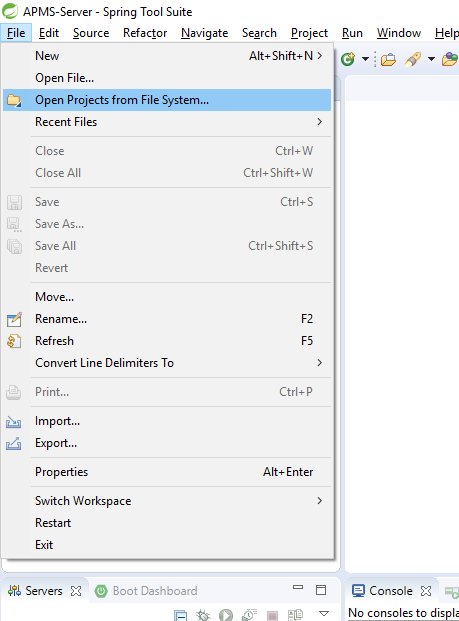
\includegraphics[width=0.7\linewidth]{images/tecnologias/importar.png}
	\caption{Botón para ejecutar el sistema.}
\end{figure}


\begin{figure}[H]
	\centering
	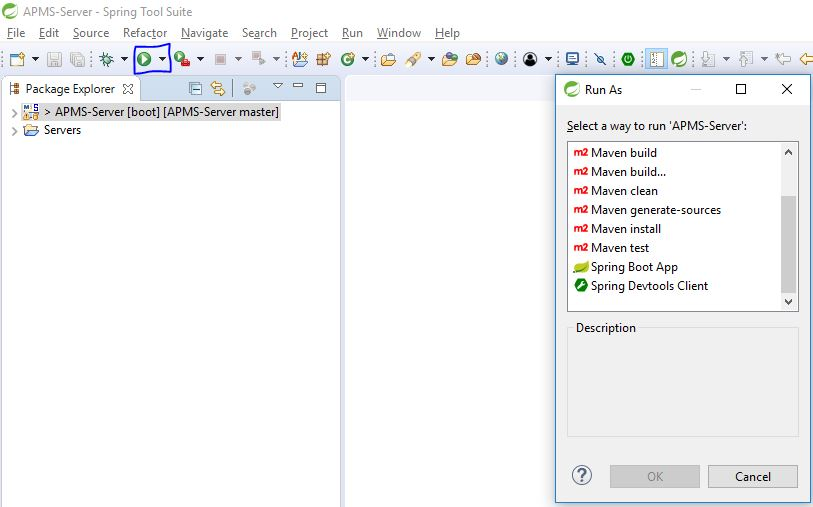
\includegraphics[width=0.7\linewidth]{images/tecnologias/correr.JPG}
	\caption{Representación gráfica de la conexión de servicios de la arquitectura del sistema.}
\end{figure}


\begin{figure}[H]
	\centering
	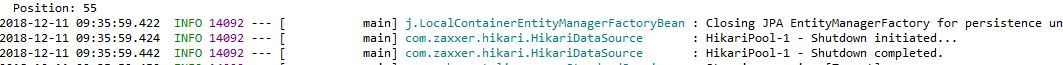
\includegraphics[width=0.7\linewidth]{images/tecnologias/springC.JPG}
	\caption{Representación gráfica de la conexión de servicios de la arquitectura del sistema.}
\end{figure}


\subsection{Angular}